\documentclass{article}

\renewcommand{\refname}{V \quad Bibliografía}
\usepackage[utf8]{inputenc}

\usepackage{multicol}
\usepackage{sectsty}
\usepackage[affil-it]{authblk}
\usepackage{graphicx}
\usepackage{url}
\usepackage[hidelinks]{hyperref}
\setlength{\columnsep}{4.26mm}
\usepackage{geometry}
\usepackage{courier}
\usepackage{xfrac}
\usepackage{amsmath}
\usepackage{array}
\usepackage{multirow}
\usepackage{caption}
\usepackage{gensymb}
\usepackage[superscript]{cite}
\usepackage[spanish, es-tabla]{babel}
\usepackage[export]{adjustbox}
\usepackage{float}
\usepackage[font=small,labelfont=bf]{caption}
\usepackage[fixlanguage]{babelbib}
%\bibliographystyle{babunsrt}
\spanishdecimal{.}

 \geometry{
 letterpaper,
 top=17mm,
 bottom=22.4mm,
 left=15.3mm,
 right=15.3mm,}

\sectionfont{\centering}
\renewcommand{\thesection}{\Roman{section}}
\renewcommand{\thesubsection}{\Alph{subsection}}
\renewcommand{\thesubsubsection}{\arabic{subsubsection}}

\title{$MgFe_2O_4$}
\author{Martina García Mejía, Laura Alejandra Sosa Ballen }
\affil{Universidad Nacional de Colombia \\ D.C. Bogotá, Colombia
    \\ \texttt{	\textup{mgarciamej@unal.edu.co, lsosab@unal.edu.co  }}\\
}
\date{6 de Junio 2099}

\usepackage{graphicx}
\graphicspath{ {/} }
\begin{document}

\sloppy
\maketitle
\begin{abstract}

este es un artículo
 

    \vspace{2mm}
    \textbf{Palabras Clave:}  womp 
\end{abstract}


\begin{multicols}{2}

\section{Introducción}

\subsection{Marco Teórico}





\section{Procedimiento y Montaje Experimental}
\subsection{Sintesis}
El $MgFe_2O_4$ se sintetizó por el método de co-precipitación, el cual consiste en precipitar simultáneamente los hidróxidos de los cationes a partir de una solución acuosa de sus sales, controlando el pH, la temperatura y la velocidad de agitación para favorecer una mezcla íntima y homogénea a nivel atómico. A partir de la fase precipitada se obtiene el óxido mixto mediante calcinación.

\subsubsection{Estequiometría}
La masa molar del $MgFe_2O_4$ es $M = 200.0\,\mathrm{g/mol}$, de modo que para obtener $1\,\mathrm{g}$ de producto se requieren $n = 5\,\mathrm{mmol}$ de espinela, es decir, $5\,\mathrm{mmol}$ de $Mg^{2+}$ y $10\,\mathrm{mmol}$ de $Fe^{3+}$ (relación molar $1:2$). Con las masas molares de los precursores, $M(Fe(NO_3)_3\cdot 9H_2O) = 404.0\,\mathrm{g/mol}$ y $M(Mg(NO_3)_2\cdot 6H_2O) = 256.4\,\mathrm{g/mol}$, las masas teóricas son $4.04\,\mathrm{g}$ y $1.28\,\mathrm{g}$ respectivamente; experimentalmente se pesaron $4.06\,\mathrm{g}$ de nitrato férrico y $1.31\,\mathrm{g}$ de nitrato de magnesio.

\subsubsection{Precipitación}
Los pasos seguidos fueron (cada etapa tiene un propósito concreto en la co-precipitación):

\begin{itemize}

\item Se disolvieron por separado $4.06\,\mathrm{g}$ de $Fe(NO_3)_3\cdot 9H_2O$ y $1.31\,\mathrm{g}$ de $Mg(NO_3)_2\cdot 6H_2O$, cada uno en un beaker con $25\,\mathrm{ml}$ de agua desionizada, y se agitaron durante 10 minutos a $400\,\mathrm{rpm}$ hasta disolución total. \textbf{Objetivo:} tener soluciones homogéneas de cada catión por separado, para que ningún hidróxido precipite antes de mezclar los cationes.

\item Se retiró el agitador de la solución de Mg y esta se incorporó poco a poco a la solución de hierro, para evitar gradientes locales de concentración y asegurar una mezcla uniforme de los cationes. \textbf{Objetivo:} mezclar $Mg^{2+}$ y $Fe^{3+}$ en proporción 1:2 a nivel molecular, condición necesaria para obtener el óxido mixto y no una mezcla de óxidos separados.

\item Se aumentó la agitación a $600\,\mathrm{rpm}$ durante 15 minutos. Mientras tanto se preparó el amoníaco al $30\%$, que actúa como agente precipitante. \textbf{Objetivo:} homogeneizar la mezcla binaria de cationes antes de iniciar la precipitación.

\item Se agregaron gotas de amoníaco mientras se monitoreaba el pH hasta alcanzar un valor entre 10 y 11, con la agitación disminuida a $400\,\mathrm{rpm}$. En este rango el medio es suficientemente alcalino para que $Fe^{3+}$ y $Mg^{2+}$ precipiten cuantitativamente como hidróxidos. Al hidrolizarse el $Fe^{3+}$ la solución se tornó de color café y el precipitado comenzó a granularse. \textbf{Objetivo:} precipitar simultáneamente ambos cationes como $Fe(OH)_3$ y $Mg(OH)_2$ (co-precipitación), garantizando la estequiometría 2:1 en el sólido.

\item Se aumentó la temperatura a $95^\circ C$ y se mantuvo la agitación durante $2\,\mathrm{h}$, lo que favorece la nucleación y el crecimiento de los precursores de hidróxido y acelera la maduración del precipitado. \textbf{Objetivo:} madurar el precipitado (menor solubilidad, partículas más definidas) para facilitar su lavado y evitar pérdidas de sólido.

\item Se retiró el agitador, se apagó la placa de calentamiento y se cubrió el beaker con papel aluminio con un orificio pequeño, para permitir la evaporación controlada del agua y evitar la contaminación del precipitado durante el reposo nocturno. \textbf{Objetivo:} dejar reposar y concentrar el precipitado sin que entre polvo u otros contaminantes.

\end{itemize}

Durante la adición del amoníaco se llevan a cabo las reacciones de precipitación
\begin{equation}
    Fe(NO_3)_3 + 3\,NH_4OH \rightarrow Fe(OH)_3\downarrow + 3\,NH_4NO_3
\end{equation}
\begin{equation}
    Mg(NO_3)_2 + 2\,NH_4OH \rightarrow Mg(OH)_2\downarrow + 2\,NH_4NO_3
\end{equation}
que generan una mezcla íntima de $Fe(OH)_3$ y $Mg(OH)_2$ en proporción $2:1$, junto con nitrato de amonio soluble.

\subsubsection{Lavado y secado}
Al día siguiente se realizó el lavado del precipitado para eliminar los subproductos solubles, principalmente el $NH_4NO_3$ y los excedentes de nitratos, que podrían generar porosidad o fases secundarias durante la calcinación. \textbf{Objetivo:} purificar el precursor de hidróxidos. Se efectuaron 3 lavados con agua destilada, centrifugando a $8800\,\mathrm{rpm}$ durante 7 minutos en cada ciclo y decantando el sobrenadante (la centrifugación compacta el sólido y facilita retirar el sobrenadante sin perder precipitado).

El sólido lavado se secó a $90^\circ C$ durante 12 horas para eliminar el agua absorbida, y luego se calcinó a $300^\circ C$ durante 2 horas para descomponer los hidróxidos y eliminar los restos de compuestos orgánicos y nitratos. \textbf{Objetivo:} secar sin descomponer el precursor y convertir los hidróxidos en el óxido mixto. En esta etapa el precursor se transforma según la reacción global
\begin{equation}
    2\,Fe(OH)_3 + Mg(OH)_2 \rightarrow MgFe_2O_4 + 4\,H_2O
\end{equation}

Posteriormente se maceró el material hasta obtener un polvo fino de tamaño uniforme y se calcinó a $400^\circ C$ durante 2 horas para consolidar la fase espinela deseada. \textbf{Objetivo:} homogeneizar el tamaño de partícula (mejor contacto entre granos y mejor respuesta en las mediciones de DRX/SEM) y alcanzar la temperatura mínima de formación de la espinela.

\subsubsection{Caracterización}
El polvo obtenido se sometió a las siguientes mediciones:
\begin{itemize}
    \item 24 de septiembre: espectroscopía UV-Vis-NIR para obtener la curva de reflectancia, y difracción de rayos X en el rango $2\theta = 20^\circ$ a $80^\circ$.
    \item 25 de septiembre: microscopía electrónica de barrido (SEM).
    \item Finalmente se recalcinó a $600^\circ C$ durante 2 horas para mejorar la cristalinidad de la fase espinela y se repitió la medición de DRX.
\end{itemize}










\subsection{SEM}
El tamaño de grano promedio es de $141 \pm 2.4$ nm (mediana $132$ nm, $N = 936$ granos; ver Secci\'on~\ref{sec:analisis}).
\begin{figure}[H]
    \centering
    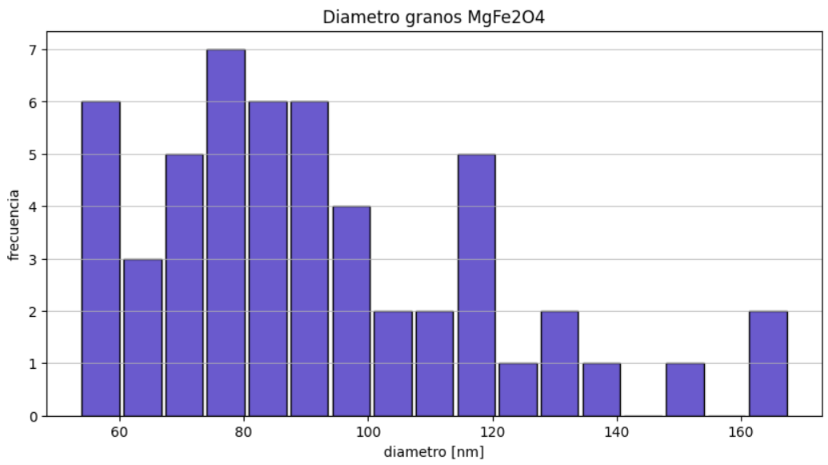
\includegraphics[scale=0.5]{assets/diametrograno.png}
    \caption{Histograma diámetro grano}
    \label{fig:histo gramo}
\end{figure}

\subsection{UVisNear}
Reflectancia difusa UV-Vis-NIR (esfera integradora): espectro limpio, an\'alisis Kubelka--Munk y gr\'aficas de Tauc con dos l\'ineas (dos fases), ver Secci\'on~\ref{sec:analisis} y Fig.~\ref{fig:tauc}.

\subsection{XDR}
Difractogramas en $2\theta = 20$--$80^\circ$ (400\ \textdegree C) y $10$--$75^\circ$ (600\ \textdegree C): identificaci\'on de fases, refinamiento Rietveld de dos fases y tama\~no de cristalito, ver Secci\'on~\ref{sec:analisis} y Figs.~\ref{fig:hxpfit}--\ref{fig:xrdsize}.

\section{An\'alisis}
\label{sec:analisis}

El an\'alisis cuantitativo completo (extracci\'on de datos, limpieza, ajustes e incertidumbres) est\'a documentado en los cuadernos de Jupyter \texttt{sem\_grain\_analysis.ipynb}, \texttt{xrd\_rietveld\_analysis.ipynb} y \texttt{uvvis\_analysis.ipynb} (directorio \texttt{analysis/notebooks}); los proyectos de HighScore Plus con la cuantificaci\'on final est\'an en \texttt{analysis/highscore/400} y \texttt{analysis/highscore/600}.

\subsection{Identificaci\'on de fases y cuantificaci\'on (DRX)}

Los difractogramas (Cu K$\alpha$, $\lambda = 1.5406$ \r{A}) se extrajeron de los archivos \texttt{.brml} del D8 Advance y se les eliminaron picos espurios de un solo canal del detector PSD. Para la identificaci\'on de picos y fases se rest\'o un fondo con un polinomio iterativo (m\'etodo de recorte); el refinamiento Rietveld, en cambio, se realiz\'o sobre los conteos crudos con un fondo polinomial modelado. Ambas pasadas (400\ \textdegree C y 600\ \textdegree C) muestran una mezcla de hematita y espinela. La identificaci\'on de fases se hizo con HighScore Plus 3.0 (PANalytical) usando las bases de referencia incluidas en el programa; las mejores coincidencias para cada pasada fueron hematita $\alpha$-Fe$_2$O$_3$ (grupo espacial $R\bar{3}c$, picos en $2\theta = 24.1^\circ, 33.2^\circ, 35.6^\circ, 49.5^\circ, 54.1^\circ, 62.5^\circ, 64.0^\circ$) y espinela MgFe$_2$O$_4$ (magnesioferrita; picos $30.1^\circ$ (220), $35.5^\circ$ (311), $43.1^\circ$ (400), $62.7^\circ$ (440)); no se detect\'o MgO ni Mg(OH)$_2$.

El refinamiento Rietveld de dos fases se corri\'o con \textbf{HighScore Plus 3.0} (PANalytical) sobre los conteos crudos, con perfil pseudo-Voigt, fondo polinomial, doblete K$\alpha_1$/K$\alpha_2$ (raz\'on 0.5), escala y celda por fase, corrimiento cero y par\'ametros de ancho $W$; las ocupaciones se fijaron a partir de las estructuras de referencia. Las fracciones en peso se obtuvieron de las escalas con el factor est\'andar de Hill--Howard $W_p \propto S_p\,Z_p M_p V_p$. La Tabla~\ref{tab:fases} resume los resultados de HighScore Plus. Las mejores coincidencias PDF usadas fueron 96-901-5066 (hematita) y 96-900-3781 (espinela) para 400\ \textdegree C, y 96-210-1170 (hematita) y 96-900-3774 (espinela) para 600\ \textdegree C. Un modelo m\'inimo in-house (pseudo-Voigt $\eta=0.3$, un FWHM por patr\'on, pesos $1/\max(I,1)$) se us\'o solo como control cualitativo: reprodujo las mismas fases y confirm\'o la dominancia de la hematita, pero no se us\'o para cuantificaci\'on. Los picos diagn\'osticos no superpuestos --- hematita 104 a $33.2^\circ$ y espinela 220/400 a $30.1^\circ/43.2^\circ$ --- fijan la dominancia de la hematita sin ambig\"uedad. La fracci\'on de espinela es $\approx 4$--$5\%$ en peso en ambas pasadas; la recalcinaci\'on a 600\ \textdegree C no produce un cambio apreciable en la fase mayoritaria. Lo que mejora sensiblemente es la cristalinidad: el FWHM global cae de $0.474^\circ$ a $0.275^\circ$ y el tama\~no de cristalito crece de $\approx 18$ a $\approx 29$ nm. El ajuste tiene $R_{wp}=1.46$--$1.54\%$ y GOF $\approx 0.72$; como el GOF es menor que 1, la incertidumbre estad\'istica es optimista y la incertidumbre real de las fracciones es mayor que la reportada.

\begin{table}[H]
\centering\footnotesize
\setlength{\tabcolsep}{4pt}
\caption{Cuantificaci\'on de fases por Rietveld (HighScore Plus 3.0, factor Hill--Howard $S\,Z\,M\,V$) y an\'alisis de tama\~no de cristalito (Cu K$\alpha$, $\lambda = 1.5406$ \r{A}). Las fracciones y celdas provienen de HighScore Plus; FWHM y tama\~nos, del an\'alisis de picos.}
\label{tab:fases}
\begin{tabular}{lcc}
\hline
 & XRD1 (400\ \textdegree C) & XRD2 (600\ \textdegree C) \\
\hline
Hematita (\% peso) & $96.3$ & $95.3$ \\
Espinela MgFe$_2$O$_4$ (\% peso) & $3.7$ & $4.7$ \\
$R_{wp}$ / GOF & $1.46\%$ / $0.72$ & $1.54\%$ / $0.72$ \\
$a$ hematita (\r{A}) & $5.0378(8)$ & $5.0358(4)$ \\
$c$ hematita (\r{A}) & $13.759(3)$ & $13.746(1)$ \\
$a$ espinela (\r{A}) & $8.350(3)$ & $8.381(5)$ \\
FWHM global ($^\circ$) & $0.474$ & $0.275$ \\
$D_{Scherrer}$ (nm) & $18.2 \pm 0.9$ & $28.7 \pm 1.6$ \\
Williamson--Hall: $D$ (nm) & $21 \pm 5$ & $76 \pm 30$ \\
Williamson--Hall: $\varepsilon$ & $0.0006 \pm 0.0010$ & $0.0019 \pm 0.0004$ \\
\hline
\end{tabular}
\end{table}

\begin{figure}[H]
    \centering
    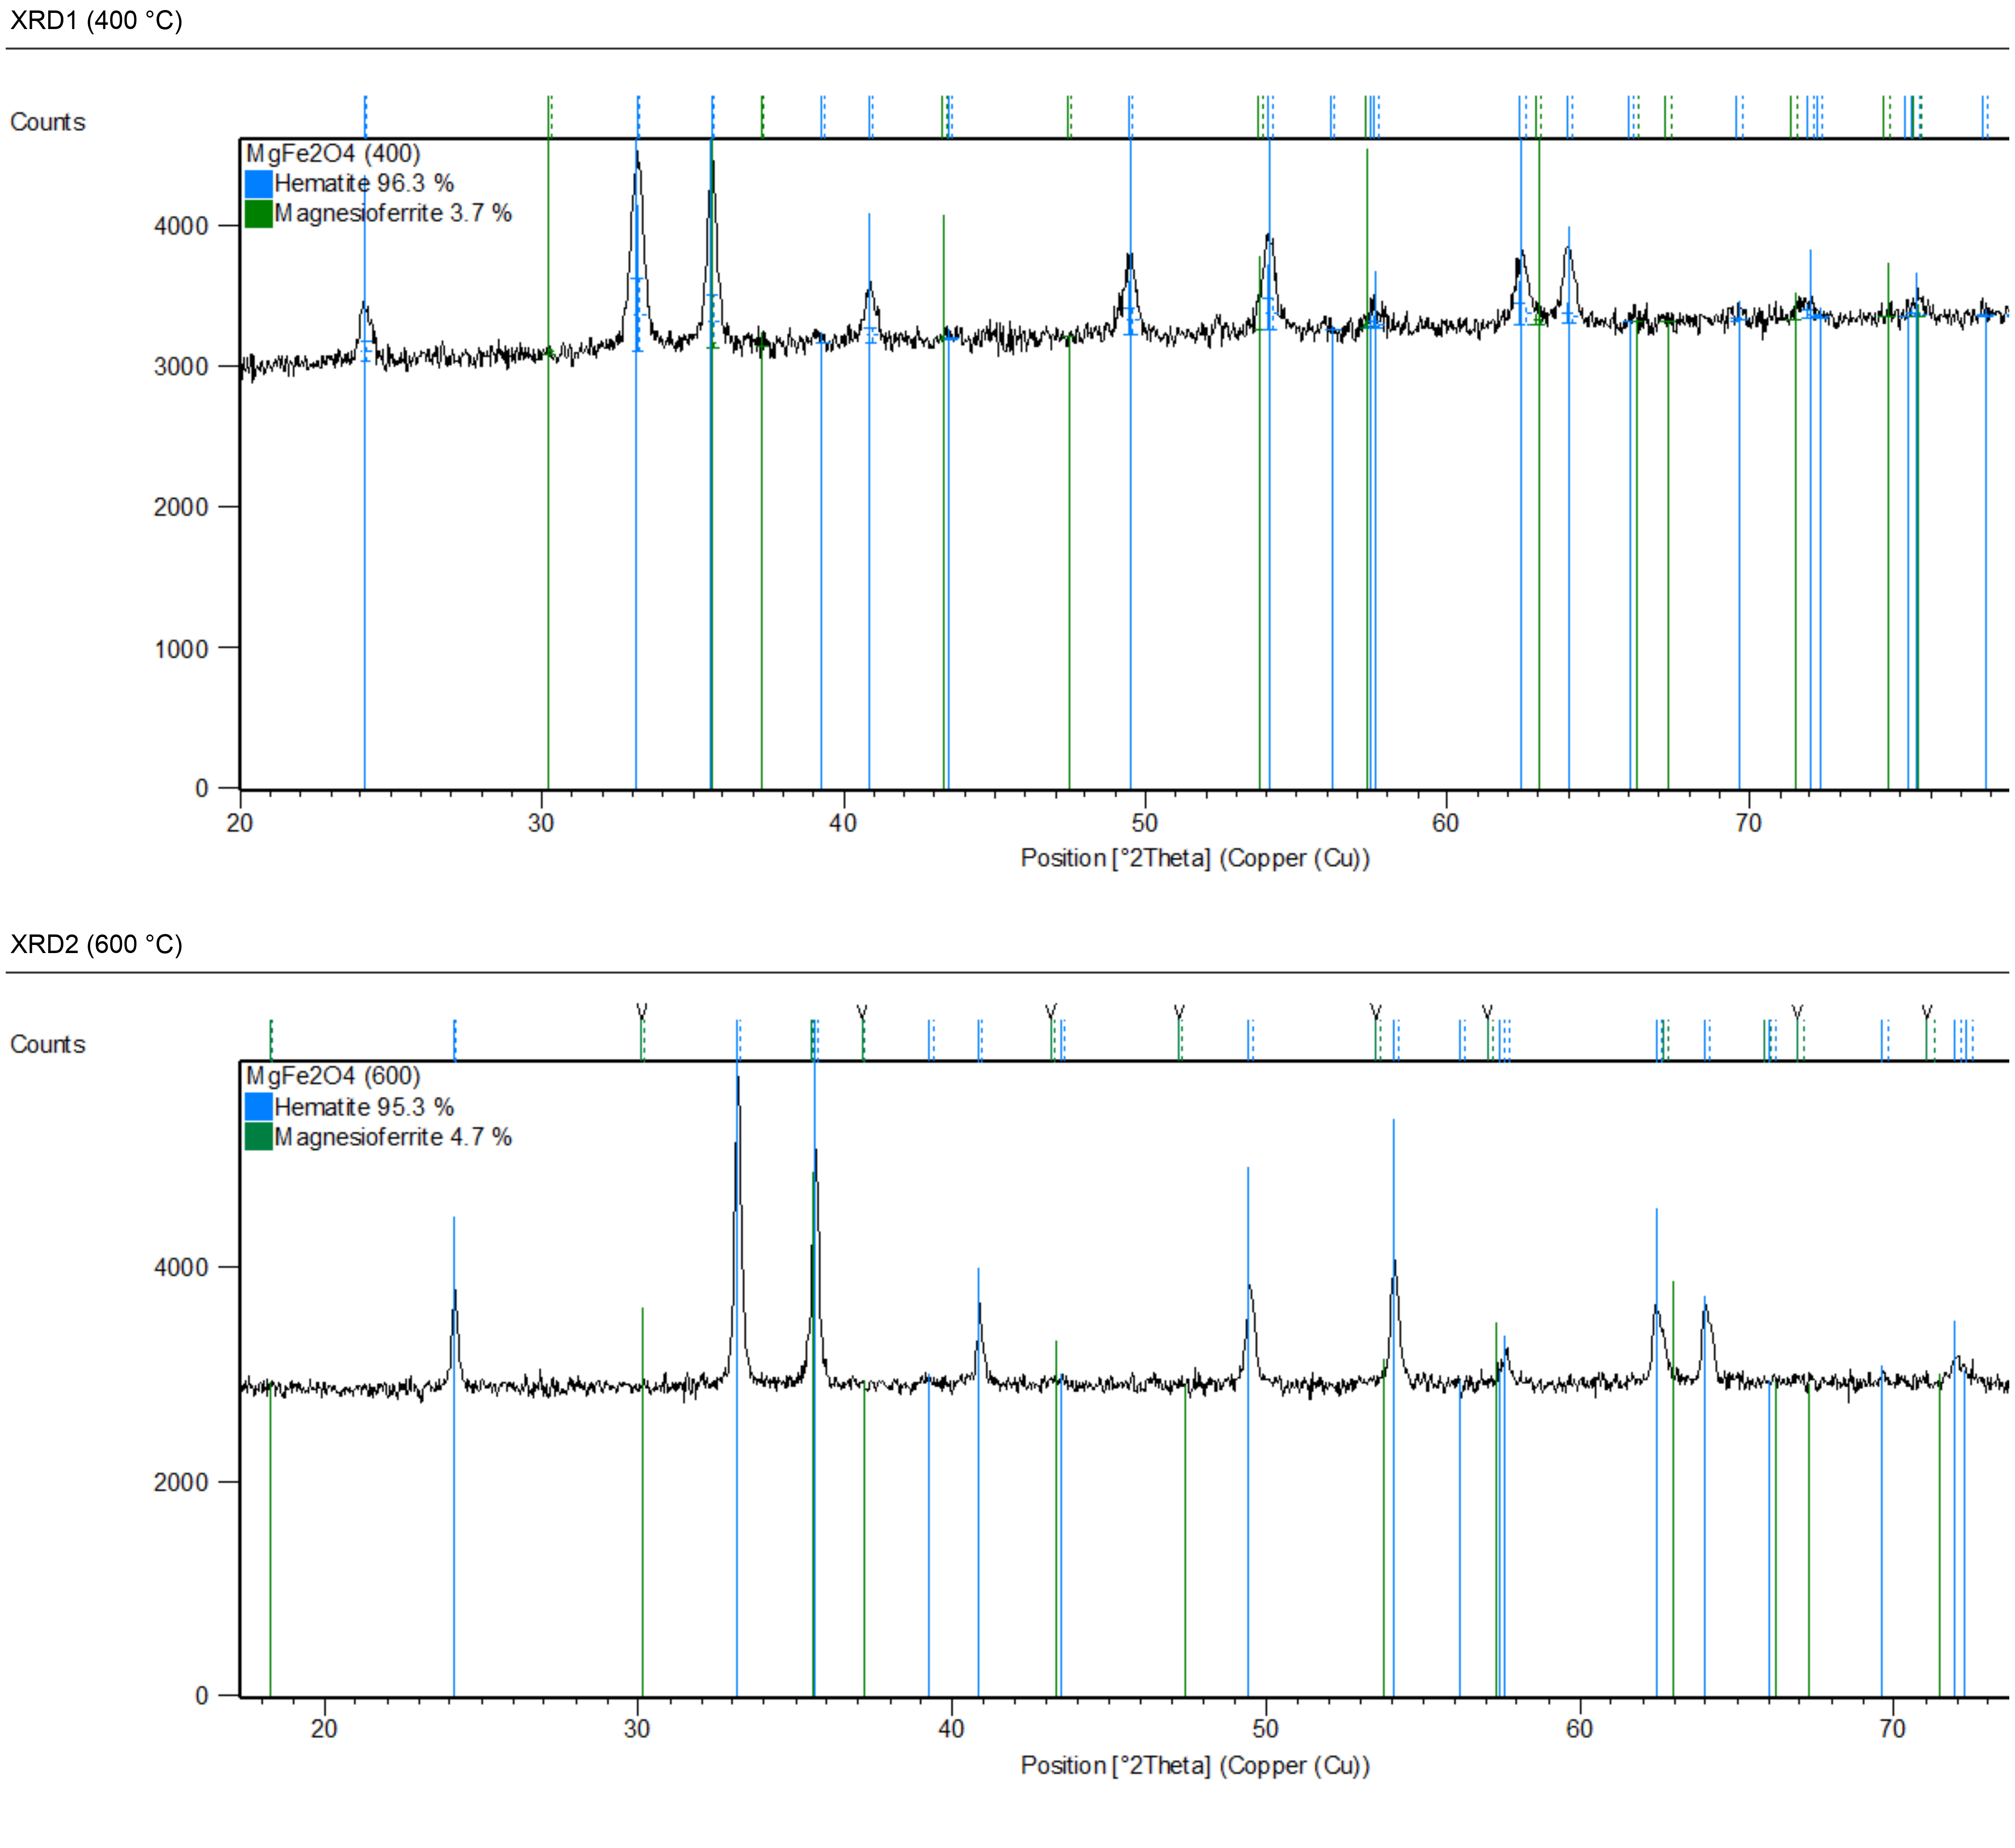
\includegraphics[width=\linewidth]{figs/xrd_highscore.png}
    \caption{Perfiles de DRX observados y posiciones de Bragg de hematita y magnesioferrita refinadas con HighScore Plus 3.0 para XRD1 (400\ \textdegree C) y XRD2 (600\ \textdegree C). Las fracciones en peso se indican en cada panel.}
    \label{fig:hxpfit}
\end{figure}

\subsection{Tama\~no de cristalito: Scherrer y Williamson--Hall}

El tama\~no de cristalito se obtuvo con la ecuaci\'on de Scherrer
\begin{equation}
    D = \frac{K\,\lambda}{\beta\cos\theta} \approx \frac{0.9\,\lambda}{\beta\cos\theta}
\end{equation}
con $\beta = \sqrt{\mathrm{FWHM}^2 - \beta_{inst}^2}$ el ancho integral corregido por el ancho instrumental ($\beta_{inst} \approx 0.05^\circ$ para D8/LynxEye). Para separar el efecto de microdeformaci\'on se us\'o el m\'etodo de Williamson--Hall,
\begin{equation}
    \beta\cos\theta = \frac{K\lambda}{D} + 4\varepsilon\sin\theta
\end{equation}
(con $\beta$ en radianes y $\lambda$ en \r{A}, $D$ en nm $= K\lambda/(\beta\cos\theta)\times 0.1$). Al graficar $\beta\cos\theta$ frente a $4\sin\theta/\lambda$, el \textbf{intercepto} es $K\lambda/D$ (tama\~no) y la \textbf{pendiente} es $\varepsilon\lambda$ (microdeformaci\'on). Los resultados por reflexi\'on (Tabla~\ref{tab:fases}) muestran crecimiento de $D \approx 18$ nm a $D \approx 29$ nm (Scherrer) con la recalcinaci\'on; en Williamson--Hall, a 600\ \textdegree C $D \approx 76 \pm 30$ nm y $\varepsilon \approx 0.0019 \pm 0.0004$, mientras que a 400\ \textdegree C la deformaci\'on no es resoluble ($\varepsilon = 0.0006 \pm 0.0010$, compatible con cero): el ensanchamiento est\'a dominado por el tama\~no de cristalito.

\begin{figure}[H]
    \centering
    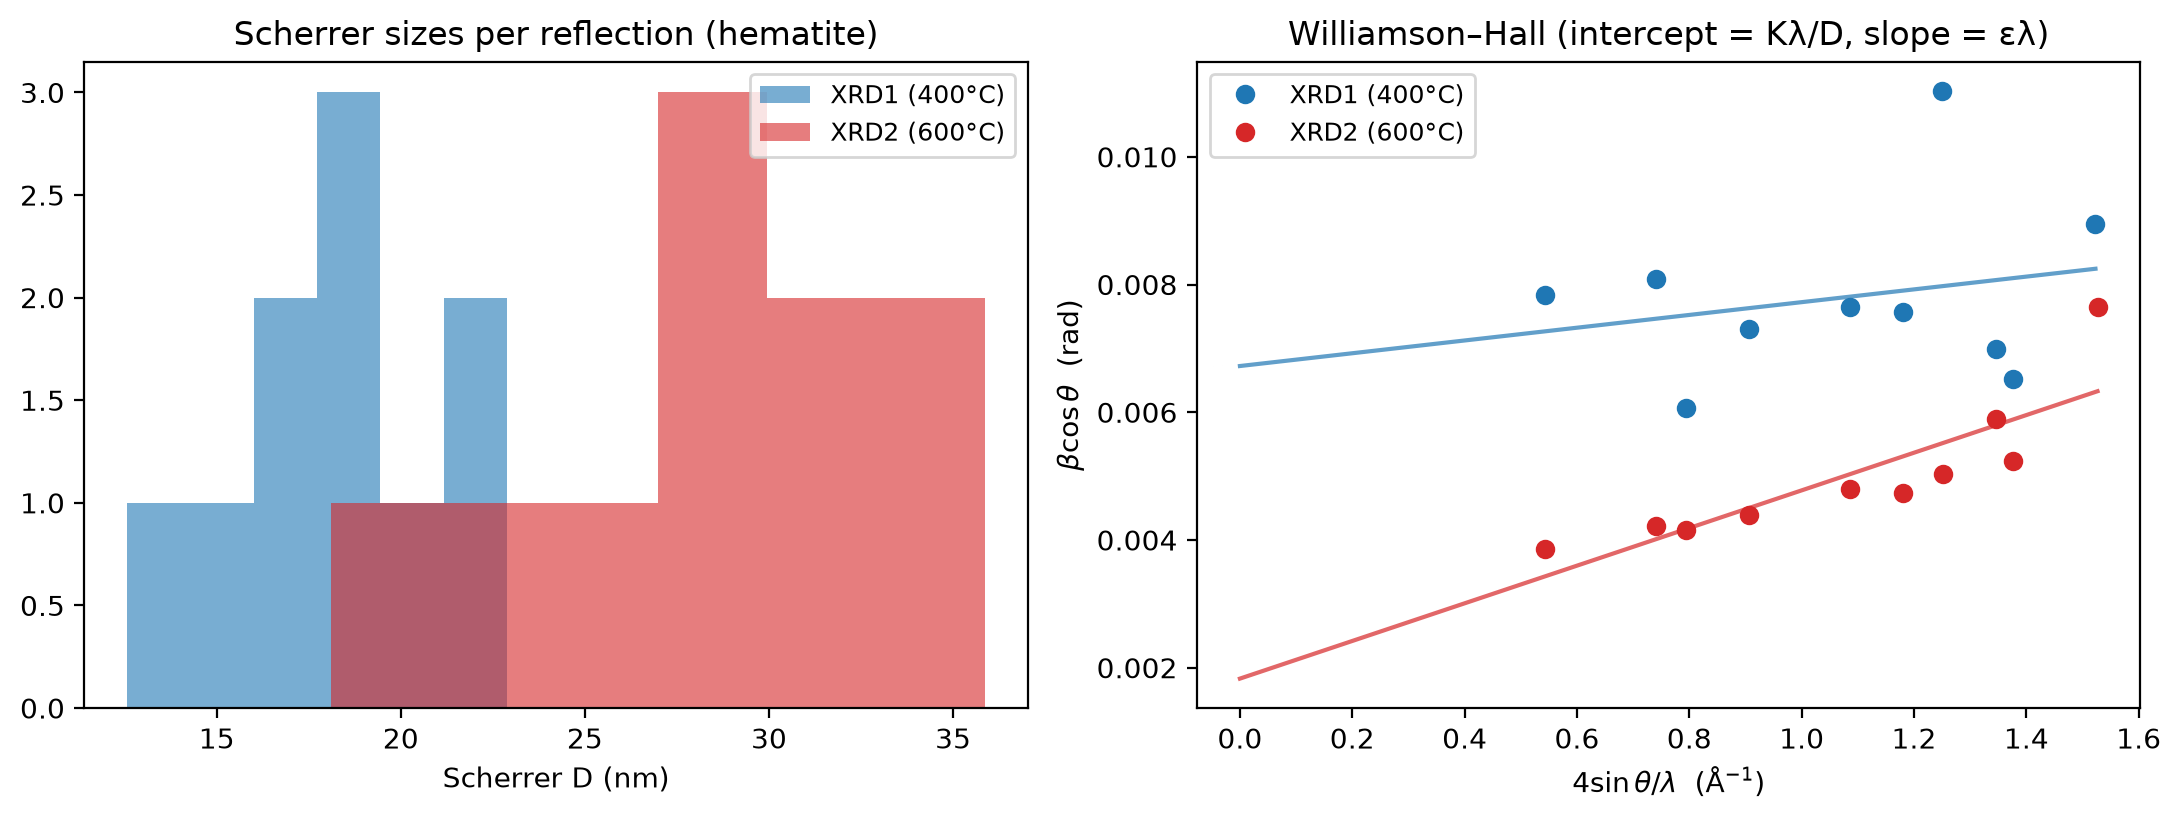
\includegraphics[width=\linewidth]{figs/xrd_size.png}
    \caption{Izquierda: distribuci\'on de tama\~nos de Scherrer por reflexi\'on para ambas muestras. Derecha: gr\'afica de Williamson--Hall.}
    \label{fig:xrdsize}
\end{figure}

\subsection{Tama\~no de grano (SEM) y distribuci\'on}

Las micrograf\'ias (VEGA3, 20 kV) se segmentaron con el siguiente pipeline (cuaderno \texttt{sem\_grain\_analysis.ipynb}): (1) recorte de la barra de informaci\'on inferior (60 px); (2) suavizado gaussiano ($\sigma = 2$ px); (3) umbral de Otsu + cierre/apertura morfol\'ogicos para consolidar la m\'ascara de granos; (4) transformada de distancia euclidiana + m\'aximos locales (distancia m\'inima 3 px) como marcadores de un watershed que separa granos toc\'andose; (5) di\'ametro circular equivalente $d = 2\sqrt{A/\pi}$ de cada regi\'on con $d > 5$ px, convertido a nan\'ometros con el tama\~no de p\'ixel de los metadatos (13.51 nm/px a 20k$\times$; 7.51 nm/px a 36k$\times$). Las magnificaciones extremas (2k$\times$: submuestreo, 135 nm/px; 70k$\times$: pocas part\'iculas y soporte de cinta) se usan solo como verificaci\'on. Las distribuciones se ajustan bien a una lognormal; el histograma combinado de las dos mejores magnificaciones ($N = 936$ granos) da una media de $141 \pm 2.4$ nm y mediana de $132$ nm, con $d_{10} = 73$ nm y $d_{90} = 246$ nm. La incertidumbre combina estad\'istica de conteo ($s_d/\sqrt{N}$) y el l\'imite de resoluci\'on ($\approx 2$ px por grano).

\begin{figure}[H]
    \centering
    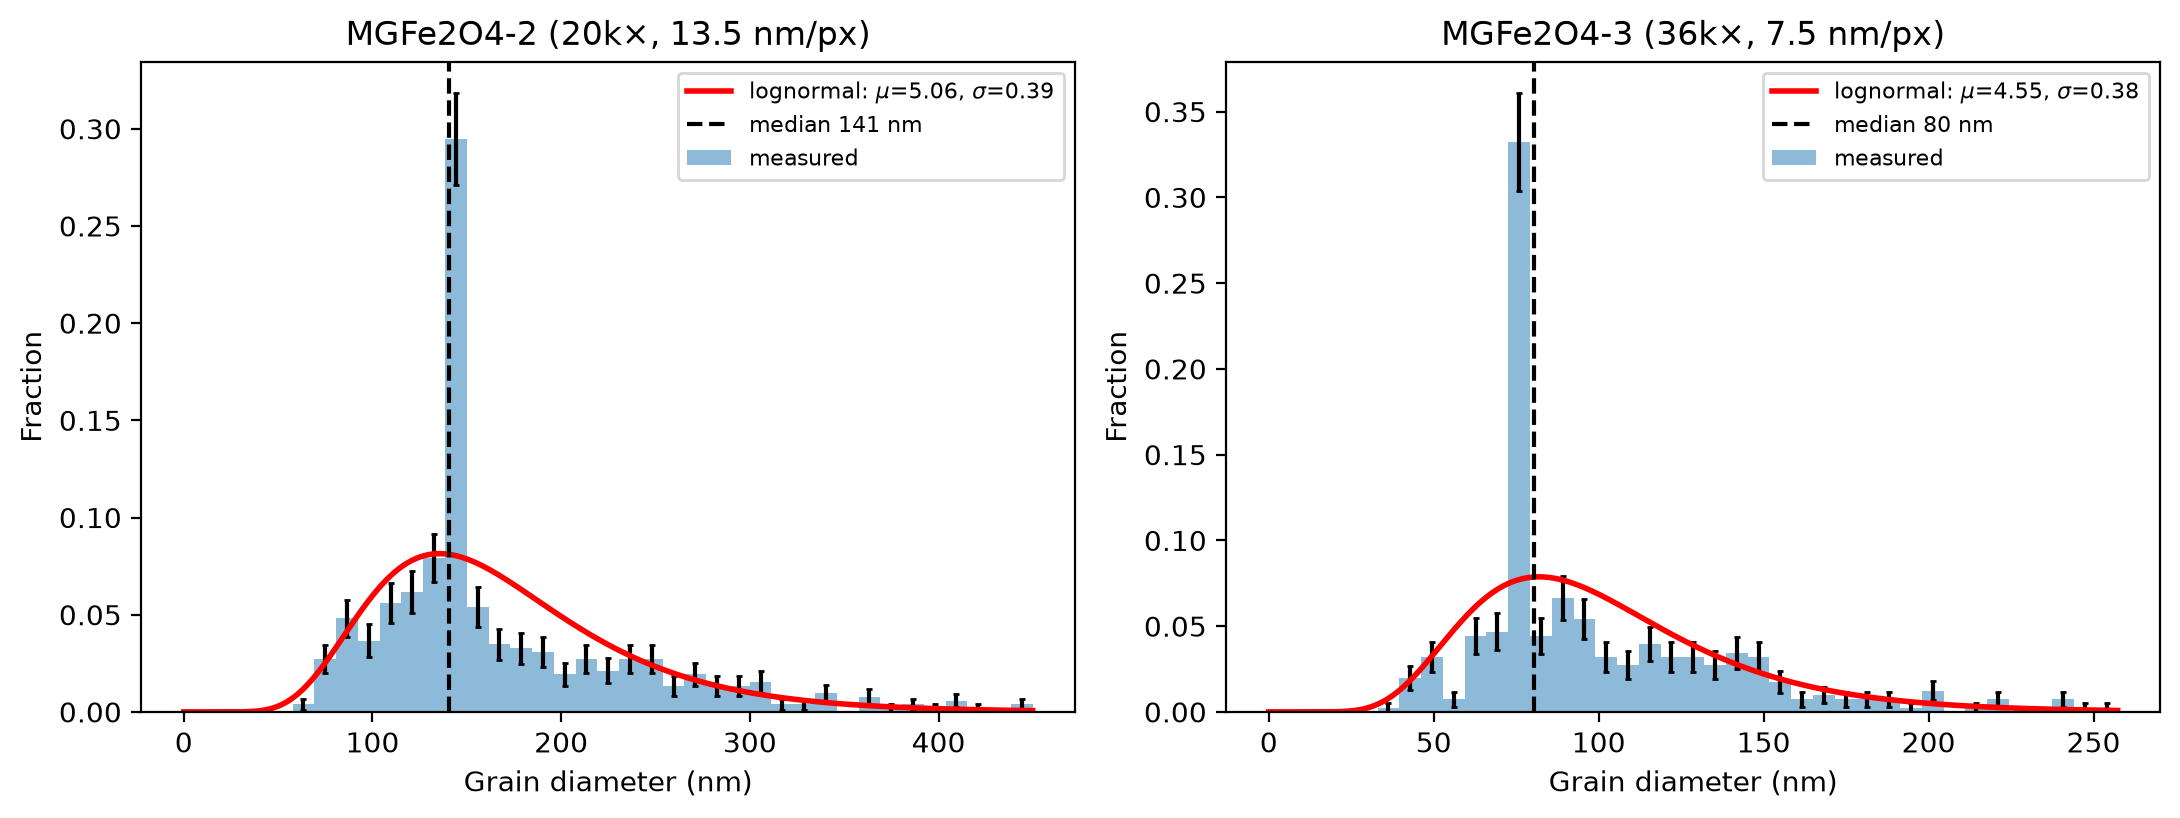
\includegraphics[width=\linewidth]{figs/sem_grain_distribution.png}
    \caption{Distribuci\'on de tama\~nos de grano con ajuste lognormal para las micrograf\'ias a 20k$\times$ y 36k$\times$.}
    \label{fig:semgrano}
\end{figure}

El tama\~no de grano de SEM ($\approx 130$--$140$ nm) es sistem\'aticamente mayor que el tama\~no de cristalito de Scherrer ($\approx 18$--$29$ nm): los granos observados son aglomerados policristalinos que contienen varios cristalitos coherentes, como es t\'ipico en polvos obtenidos por co-precipitaci\'on.

\subsection{Composici\'on y relaciones m\'asicas (EDS y UV-Vis)}

La cuantificaci\'on EDS (XFlash 410, 30 kV) embebida en el archivo \texttt{.spx} da Fe $62.3 \pm 2.6$ \% peso, O $35.7$ \% peso, C $5.7$ \% peso (atribuido principalmente a la cinta adhesiva de carbono) y Mg $0.9 \pm 1.1$ \% peso. Excluyendo el carbono, la composici\'on es Fe $63.0$ \%, O $36.1$ \%, Mg $0.9$ \% en peso. La relaci\'on m\'asica Fe:Mg medida ($\approx 69:1$) difiere de la estequiom\'etrica ($4.60:1$) porque la l\'inea Mg K$\alpha$ (1.253 keV) es pr\'oxima al l\'imite de detecci\'on y se solapa con el fondo bajo los picos de Fe, lo que subestima el Mg; adem\'as, el Mg$^{2+}$ es m\'ovil y puede perderse parcialmente en los lavados, en l\'inea con el exceso de hematita observado por DRX.

En reflectancia UV-Vis-NIR (esfera integradora), el polvo presenta $R \approx 6.5\%$ en el visible 400--700 nm (pigmento oscuro caf\'e-rojizo), bordes de absorci\'on cerca de 770--795 nm (derivada $d[F(R)]/dE$: onsets a $1.56$ y $1.62$ eV) y una meseta NIR con $R \approx 0.37$ a 1500--2500 nm. La gr\'afica de Tauc muestra \textbf{dos l\'ineas rectas}, que corresponden a las \textbf{dos fases} cuantificadas por DRX, no a dos exponentes de un mismo borde: la l\'inea de la espinela MgFe$_2$O$_4$ a $E_g \approx 1.6$--$1.7$ eV ($1.63 \pm 0.02$ eV, ajuste con $n=1/2$ en 1.9--2.3 eV) y la l\'inea de la hematita $\alpha$-Fe$_2$O$_3$ a $E_g \approx 2.0$ eV ($2.00 \pm 0.03$ eV, ajuste con $n=2$ en 2.0--2.4 eV), en acuerdo con los valores de la literatura (hematita $\approx 2.0$--$2.2$ eV; MgFe$_2$O$_4$ $\approx 1.6$--$1.9$ eV). Al ser la hematita la fase mayoritaria, su se\~nal domina el espectro.

\begin{figure}[H]
    \centering
    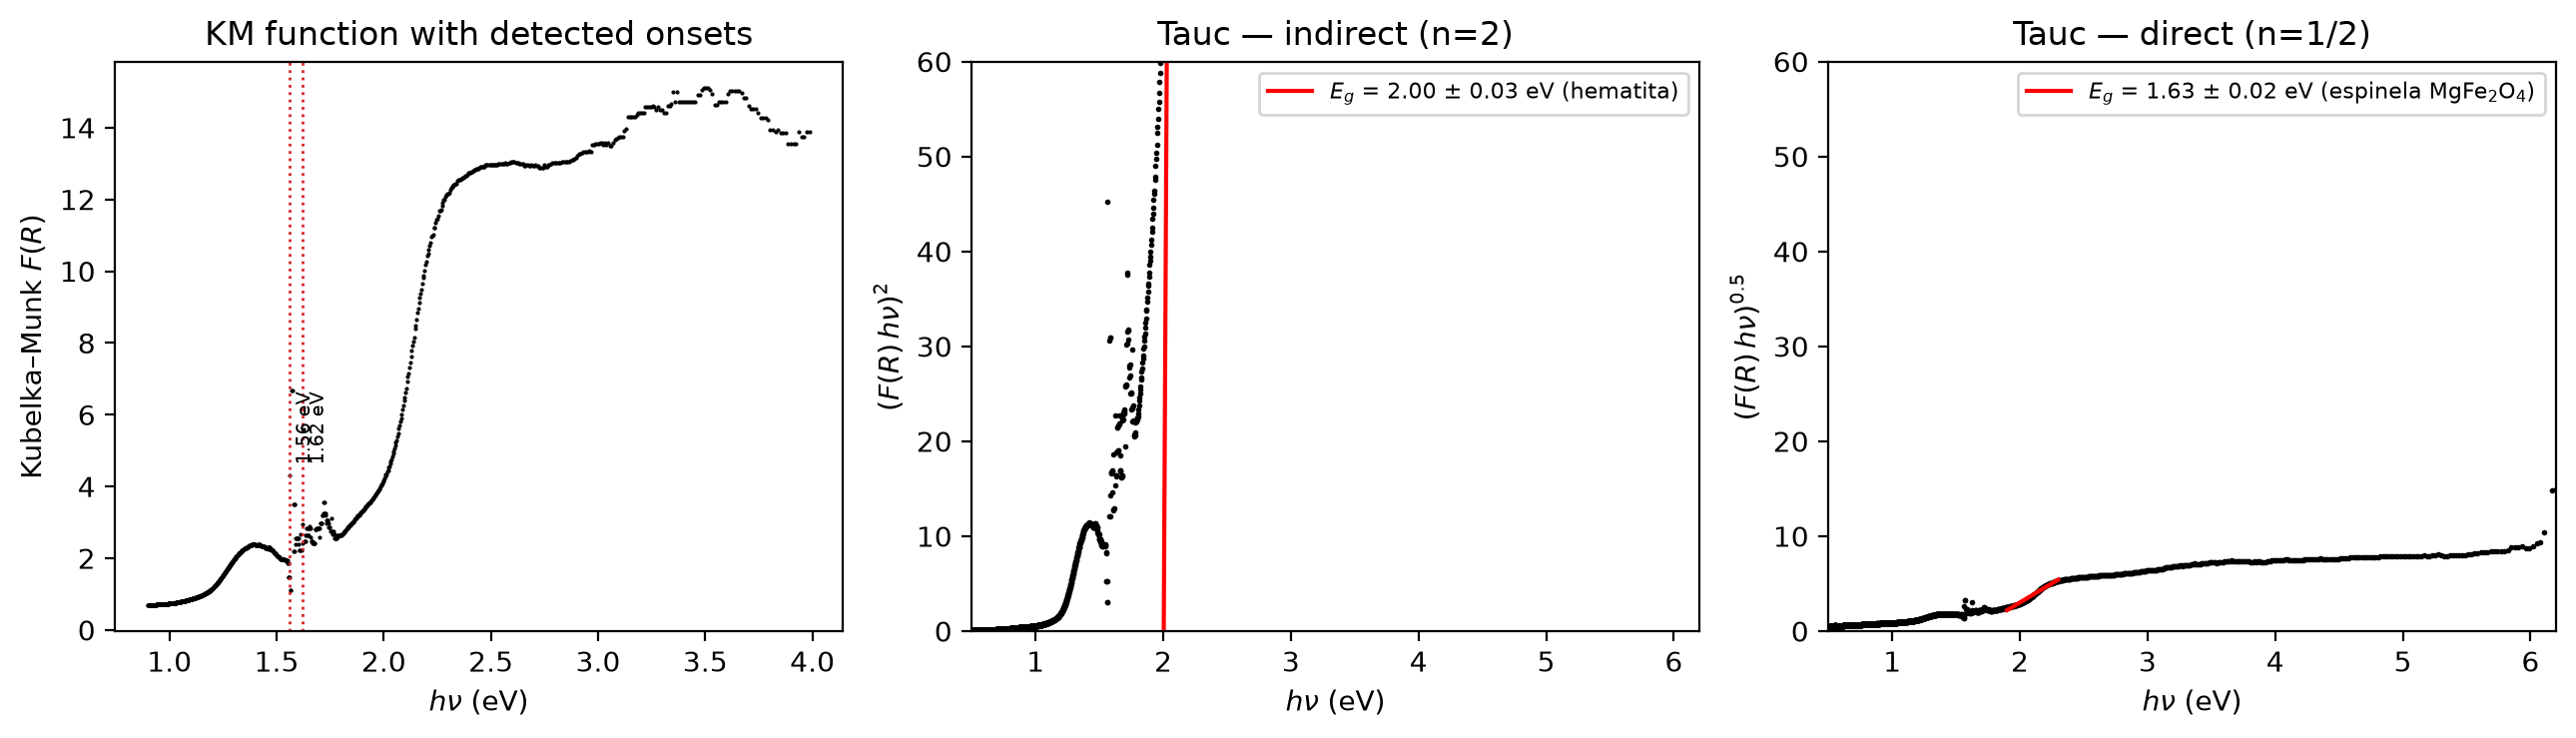
\includegraphics[width=\linewidth]{figs/uvvis_tauc.png}
    \caption{An\'alisis de Tauc del espectro limpio de reflectancia: dos l\'ineas correspondientes a las dos fases (espinela MgFe$_2$O$_4$ $\approx 1.6$ eV y hematita $\approx 2.0$ eV).}
    \label{fig:tauc}
\end{figure}

\begin{figure}[H]
    \centering
    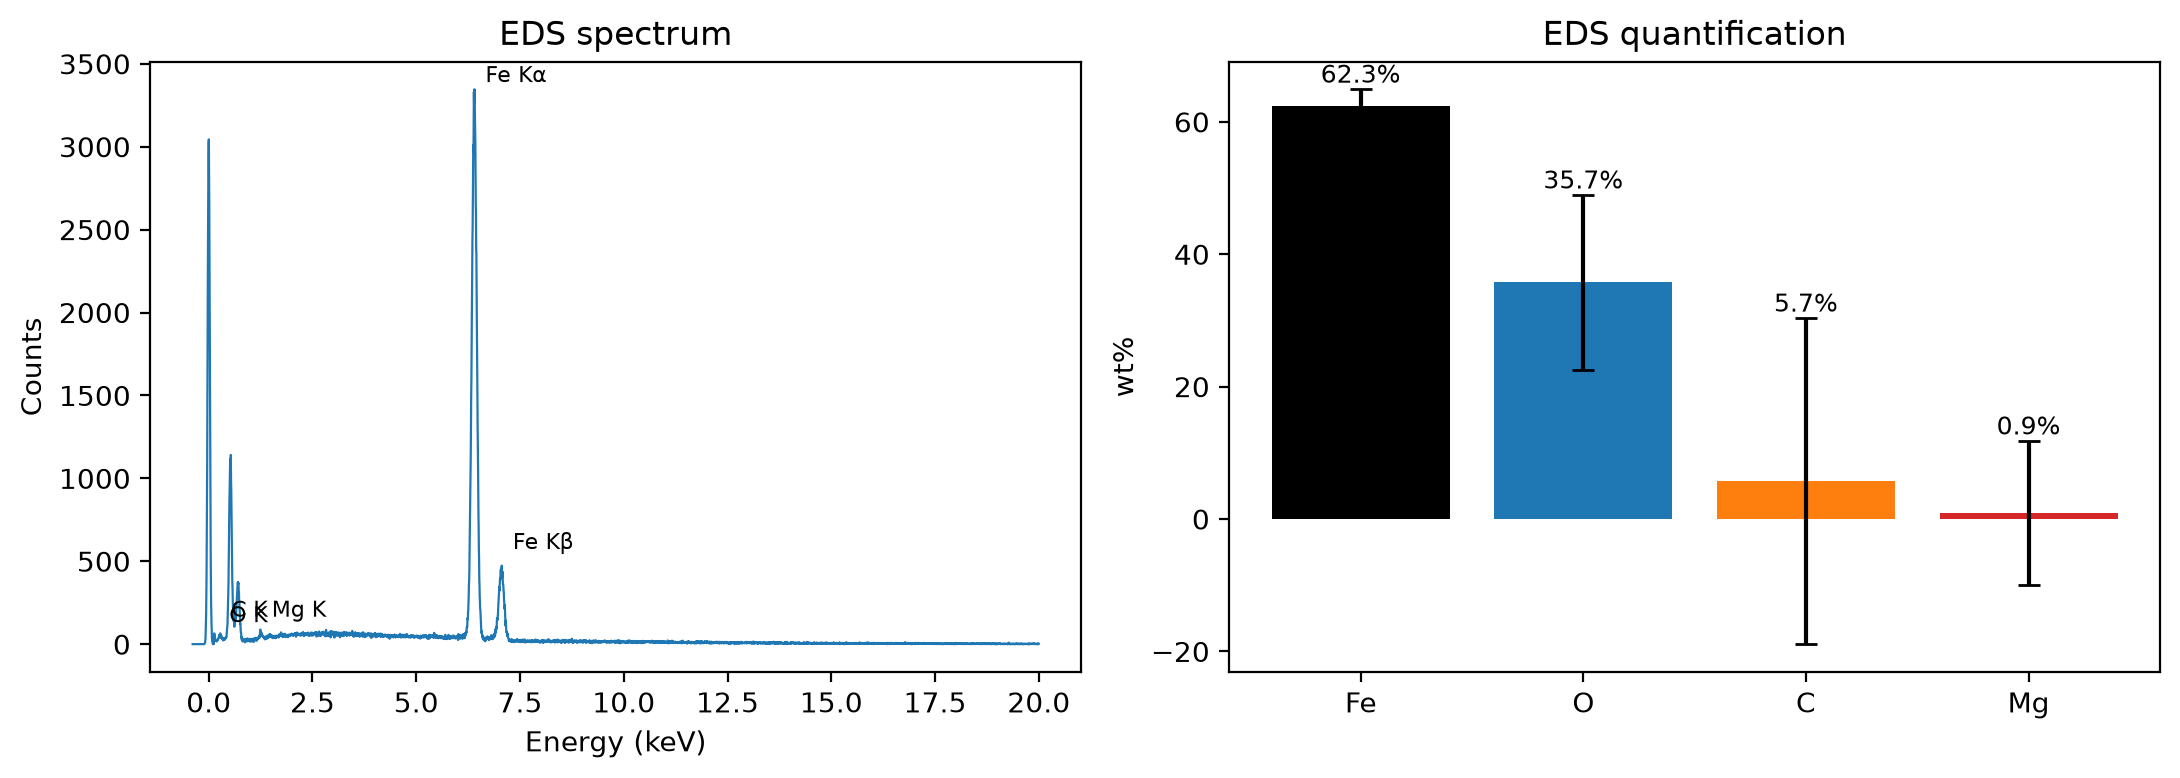
\includegraphics[width=0.9\linewidth]{figs/sem_eds.png}
    \caption{Espectro EDS con las l\'ineas identificadas y cuantificaci\'on en \% peso.}
    \label{fig:eds}
\end{figure}

\subsection{S\'intesis de resultados}

\begin{itemize}
    \item La muestra s\'intetizada por co-precipitaci\'on y calcinada a 400\ \textdegree C / 600\ \textdegree C NO es espinela pura: es una mezcla $\approx 95$--$96\%$ hematita + $\approx 4$--$5\%$ espinela MgFe$_2$O$_4$ (Rietveld de dos fases con HighScore Plus 3.0, $R_{wp}=1.46$--$1.54\%$, GOF $\approx 0.72$), coherente con el color caf\'e-rojizo y las dos l\'ineas del Tauc.
    \item La recalcinaci\'on a 600\ \textdegree C no altera apreciablemente la fase mayoritaria; la espinela permanece minoritaria ($\approx 4$--$5\%$ en peso), pero mejora la cristalinidad: FWHM global $0.474^\circ \rightarrow 0.275^\circ$ y cristalitos de $\approx 18$ a $\approx 29$ nm (Scherrer); la microdeformaci\'on W--H pasa a ser mensurable ($\varepsilon \approx 0.0019$).
    \item Los granos de SEM (media $141 \pm 2.4$ nm, mediana $132$ nm) son aglomerados de $\sim$5--7 cristalitos DRX.
    \item El Tauc muestra dos l\'ineas = dos fases: espinela $\approx 1.6$ eV y hematita $\approx 2.0$ eV.
    \item EDS subestima el Mg (relaci\'on Fe:Mg $\approx 69:1$ vs $4.6:1$ estequiom\'etrica); el Mg remanente est\'a en la fase espinela detectada por DRX.
\end{itemize}

Pr\'oximos pasos:
\begin{itemize}
    \item Repetir la s\'intesis controlando mejor el pH y la temperatura de calcinaci\'on para aumentar la fracci\'on de espinela (objetivo: espinela mayoritaria).
    \item Cuantificar el Mg por una t\'ecnica sensible (ICP) para cerrar el balance m\'asico.
    \item Refinar con HighScore Plus a\~nadiendo orientaci\'on preferida (March--Dollase) y par\'ametros de tama\~no/deformaci\'on.
\end{itemize}



En la siguiente figura se puede observar el montaje: 

\begin{figure}[H]
    \centering
    
\includegraphics[scale=0.13]{assets/ensayo.png}
    \caption{Montaje Experimental}
    \label{fig:Hielo}
\end{figure}

\bibliographystyle{ieeetr}
\bibliography{refs.bib}

\end{multicols}   


\centering
\maketitle
\end{document}